\documentclass[xcolor=dvipsnames]{beamer}

\usepackage[utf8]{inputenc}
\usepackage[french]{babel}
\usepackage{url}
\usepackage{lmodern}
\usepackage{listings}
\usepackage{graphicx}
\usepackage{xcolor}
\usepackage{textcomp} 
\usepackage{hyperref}
%% \usepackage{subcaption}
\usepackage[T1]{fontenc}
\usepackage{graphicx}
\usepackage{verbatim}
\usepackage{color}
 
\setbeamertemplate{footline}{\hspace*{.5cm}\scriptsize{\insertauthor\hspace*{50pt} \hfill\insertframenumber\hspace*{.5cm}}}


\setbeamertemplate{section in toc}{%
\textcolor{MidnightBlue}{$\blacktriangleright$ \inserttocsection}
}

\AtBeginSection[]
{
  \begin{frame}<beamer>{}
    \tableofcontents[currentsection,hideothersubsections]
  \end{frame}
} 

\usecolortheme{seahorse}
\usecolortheme{rose}
\useoutertheme{infolines}

\usecolortheme[named=SkyBlue]{structure}
\setbeamercolor{block title}{fg=MidnightBlue}

\title[Nominal Workbench]{Nominal Workbench\\Système de Réécriture Nominale}

\author[\'Equipe NoWork]{Rémy B. Yohan B. Vincent B. Mathieu C. Pierrick C. Matthieu D. Roven G. I\~nigo M. Pierre T.}

\institute[UPMC]{Université Pierre et Marie Curie}

\date{Jeudi 20 mars 2014}

\begin{document}

\begin{frame}
\titlepage
\end{frame}

%% Recette

%% présentation générale du système de réécriture / architecture
%% Rémy
\section{Introduction}
%% présentation générale
%% architecture





\begin{frame}{Introduction}

  \begin{block}{Rewriting system}

    A method to modelize, in general, the operations of replacing
    subterms in a term by others.\\
    ~\\

    \emph{ie. reduction step of a language semantic, propositionnal
      logic De Morgan's laws, Peano's arithmetic}
    
  \end{block}

  
\end{frame}

\begin{frame}{Rewriting system}

  \begin{block}{Definition}
    
    \begin{itemize}
      \item a set of terms 
      \item a set of rules (term * term)
    \end{itemize}

  \end{block}

  Rewrite a term : applying rules according to a predefined
  \textcolor{red}{strategy} on a given term by \textcolor{blue}{matching} and \textcolor{blue}{replacing} its subterms.

  ~\\
  For instance : \\
  Rule : \texttt{Sub(Add(X))} $\rightarrow$ \texttt{X}\\
  ~\\
  \textcolor{blue}{\texttt{Sub(Add(0))}} $ \rightarrow $ \textcolor{blue}{\texttt{0}}

\end{frame}


\begin{frame}{Non-Linear Nominal Rewriting}
  
  \begin{block}{Nominal}
    There is a distinction between atoms (variables of the language)
    and placeholders/meta-variables (the suterm to replace).
  \end{block}

  \begin{block}{Non-Linear}
    Two instances of the same placeholder
    can appear in the left-hand side of the rule. 
  \end{block}
  
\end{frame}



\begin{frame}{\textcolor{red}{No}minal \textcolor{red}{Work}bench}

  The only rewriting workbench implementing : \\
  \textcolor{blue}{non-linear pattern matching} + \textcolor{blue}{nominal rewriting}

  \begin{block}{Features}
  \begin{itemize}
    \item \textcolor{red}{A simple language} for rewriting systems
    \item Write complexe \textcolor{red}{strategies} with an
      expressful language
    \item Run rewriting operations on terms in an \textcolor{red}{interactive top-loop}
  \end{itemize}
  \end{block}
  
\end{frame}


\begin{frame}{Architecture}

\begin{figure}[h]
\begin{center}
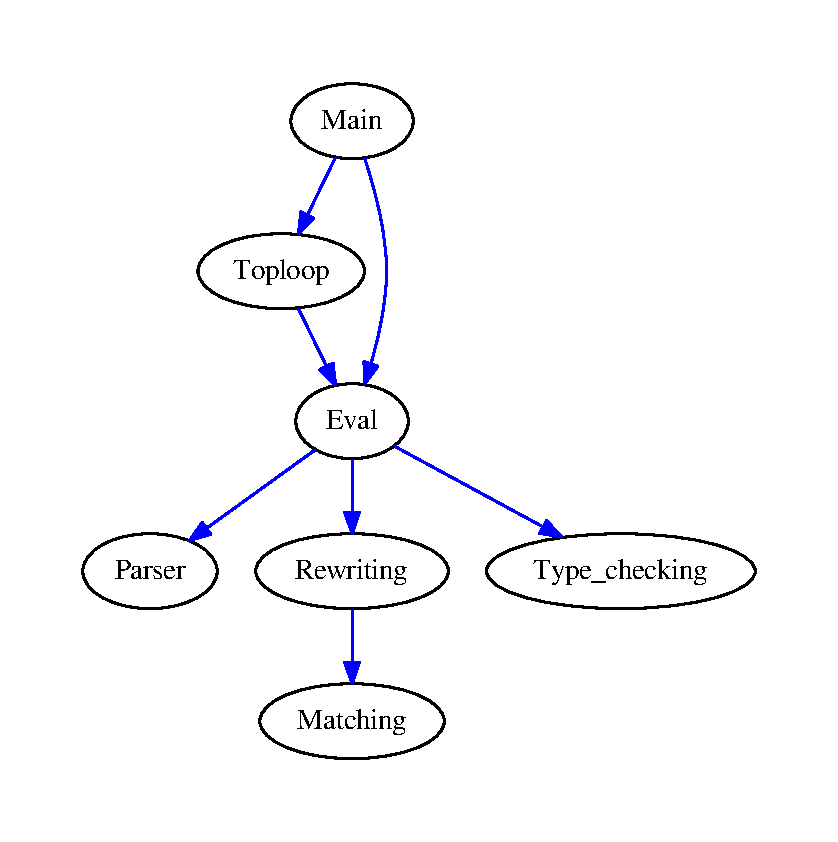
\includegraphics[ height=0.9\textheight]{imports/architecture.pdf}
\end{center}
\end{figure}

\end{frame}


\begin{frame}{Abstract Syntax Trees Architecture}

\begin{figure}[h]
\begin{center}
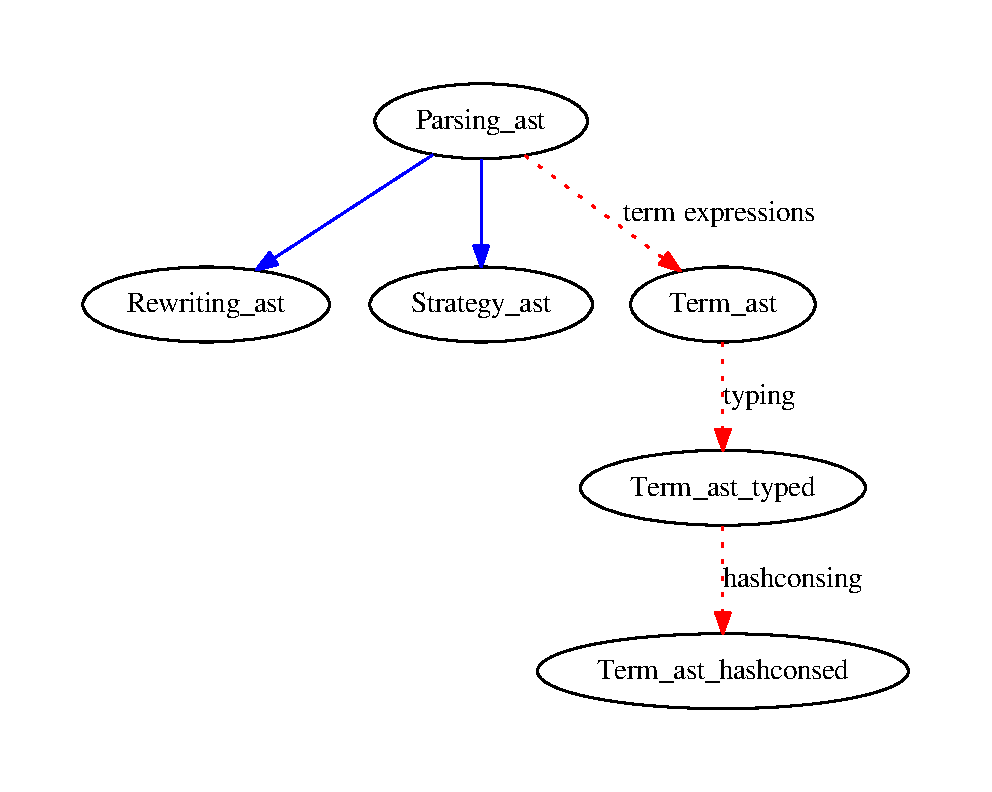
\includegraphics[ height=0.7\textheight]{imports/asts.pdf}
\end{center}
\end{figure}

\end{frame}


%% syntaxe/langage du bouzin
%% Matthieu
\section{Langage}
\begin{frame}{Description d'un système de réécriture}
  \begin{block}{Description}
    La description d'un système se fait par des déclarations de 4
    sortes différentes :
    \begin{itemize}
    \item \verb?kind?
    \item \verb?constant?
    \item \verb?operator?
    \item \verb?rule?
    \end{itemize}
  \end{block}
\end{frame}

\begin{frame}[fragile]{Kind}

  Le mot-clé \verb?kind? pour décrire les types manipulés par le
  système de réécriture.
\begin{verbatim}
  kind Integer : type
  kind List : type -> type
  kind Couple : type -> type -> type
  kind Var : atom
\end{verbatim}
\end{frame}

\begin{frame}[fragile]{Constant}
  \begin{itemize}
  \item élément de base du langage
  \item typé avec les types du langage décrit (\verb?kind?)
  \end{itemize}

\begin{verbatim}
  kind Integer : type
  kind Bool : type
  kind List : type -> type
  kind Couple : type -> type -> type

  #generics
  constant Nil : forall(A).List<A>
  constant NilAssoc : forall(A,B).List<Couple<A,B>>

  #instatiated
  constant IntNil : List<Integer>
\end{verbatim}
\end{frame}

\begin{frame}[fragile]{Operator}
  Déclarations similaires aux déclarations de constantes.
\begin{verbatim}
  operator Cons : forall(A).A * List<A> -> List<A>
  operator Hd : forall(A).List<A> -> A
  operator Tl : forall(A).List<A> -> List<A>

  # Hd(Tl(Cons(False, Cons(True, Nil))))
\end{verbatim}
\end{frame}

\begin{frame}[fragile]{Rule}
  \begin{itemize}
  \item L'ordre d'application des règles est définit par les stratégies
  \item Généricité structurelle (\emph{placeholders})
  \end{itemize}

  \begin{verbatim}
    rule [hd]:
      Hd(Cons(?x, ?y)) => ?x

    rule [tl]:
      Tl(Cons(?x, ?y)) => ?y
  \end{verbatim}
\end{frame}


%% type-checking
%% Mathieu Matthieu
\section{Typage}
\begin{frame}{Typage - Bases}

\begin{itemize}
\item Pas de symbole inconnu
\smallskip
\item Arités des applications correctes (kinds, opérateurs)
\smallskip
\item On ne peut pas appliquer un type générique
\smallskip
\item Pas d'atom dans un kind \emph{flèche} %à reformuler
\smallskip
\item Binders de kind atom
\end{itemize}

\end{frame}

\begin{frame}{Typage des règles}

Tous les \emph{placeholders} de l'effet apparaissent dans le pattern
\medskip

On veut parcourir le pattern puis l'effet avec un environnement comprenant :
\smallskip

\begin{itemize}
\item les types des \emph{placeholders}
\item les instanciations de types génériques
\end{itemize}
\bigskip

\textit{Exemple :}
\linebreak
\texttt{operator O : forall(A). A * A -> A}
\linebreak
\texttt{rule [r] : O(C1, C2) => C1}

\end{frame}

\begin{frame}{Typage - Unification}

\textbf{Problème :} gérer les types génériques lors du parcours en profondeur d'un terme
\medskip

\textit{Exemple :}\linebreak
\texttt{operator O : forall(A). A * B -> A}\linebreak
\texttt{rule [r] : O(O(C1,C2), C2) => C1}% avec type(C1) != type (C2)
\medskip

\textbf{Idée :} 
\begin{itemize}
\item l'environnement pour les types génériques n'est valable que pour un niveau
\item notion d'équivalence entre types (\textit{forall(A).A $\approx$ forall(B).B})
\item renommage de type
\end{itemize}

\end{frame}


%% pattern-matching / hash-consing
%% Pierrick
\section{Pattern Matching}

\begin{frame}

\'Elément principal de la réécriture nominal : pattern matching. Indique si un
terme est de la forme d'un \emph{pattern} (motif) donné, et en extrait des informations

\bigskip

Deux types de pattern matching : 
\begin{itemize}
\item Linéaire. 
\item Non linéaire. 
\end{itemize}

\end{frame}

\subsection{Pattern matching linéaire}


\begin{frame}
\frametitle{Exemple de pattern matching}

Prenons ce terme :
\texttt{Lambda(x, Var(x))}. 
\begin{itemize} 

  \item matche \texttt{Lambda(\_, \_)}.
  \item mais pas \texttt{Var(\_)}.

\end{itemize}

\bigskip

Extraction de sous-termes :

\texttt{Lambda(?x, \_)} retourne le sous-terme correspondant à \emph{?x}.

\end{frame}

\begin{frame}
\frametitle{Concrètement}

Exemple du déroulement du pattern-matching:
\begin{itemize}
  
  \item Terme : \texttt{Lambda(y, Var(y))}.

  \item Pattern : \texttt{Lambda(\_, Var(?x))}.

\end{itemize}

\bigskip

\begin{center}
  \only<2>
      {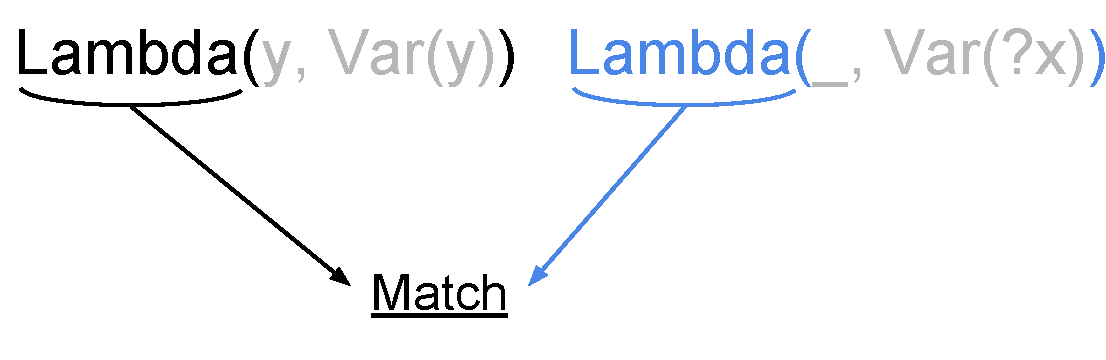
\includegraphics[scale=0.5]{pattern/trivial1.pdf}}
  \only<3>
      {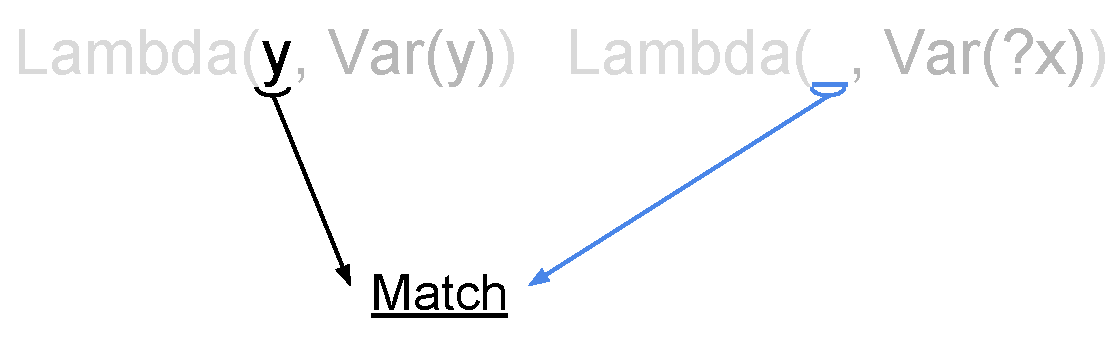
\includegraphics[scale=0.5]{pattern/trivial2.pdf}}
  \only<4>
      {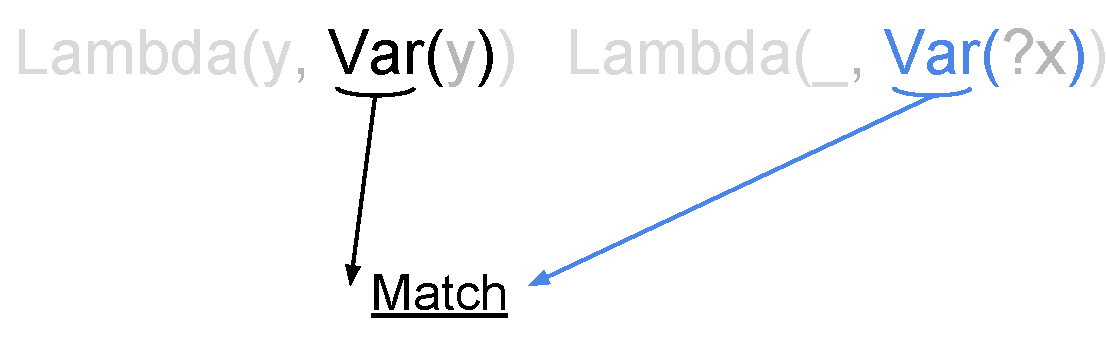
\includegraphics[scale=0.5]{pattern/trivial3.pdf}}
  \only<5>
      {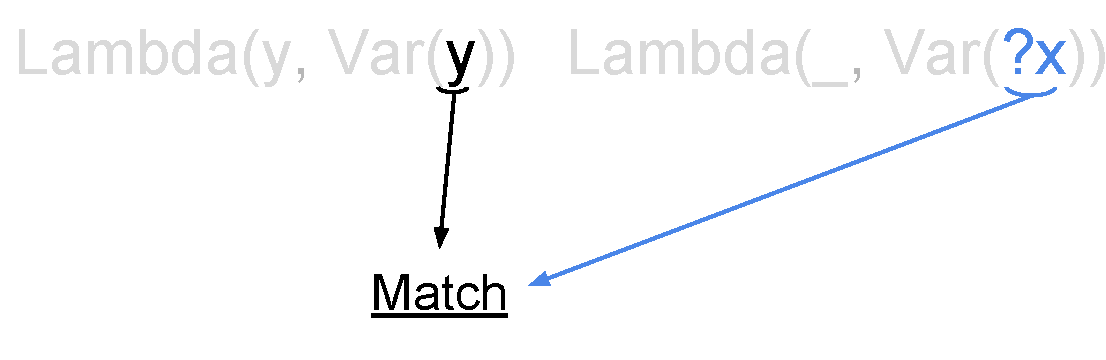
\includegraphics[scale=0.5]{pattern/trivial4.pdf}}
  \only<6>
      {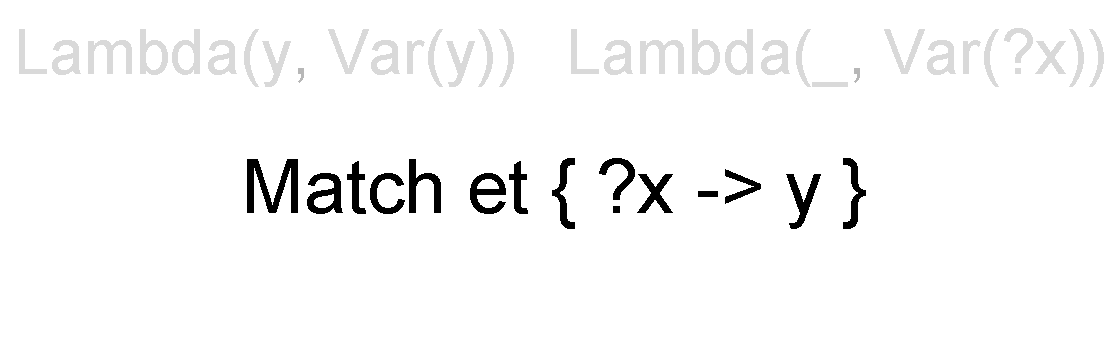
\includegraphics[scale=0.5]{pattern/trivial5.pdf}}

\end{center}

\end{frame}

\begin{frame}
\frametitle{Non linéarité des atomes}

Possibilité de matcher deux atomes liés même dans le cas linéaire.

Par exemple avec \texttt{Lambda(?x, Var(?x))} :

\bigskip
\begin{center}
  \only<2>
      {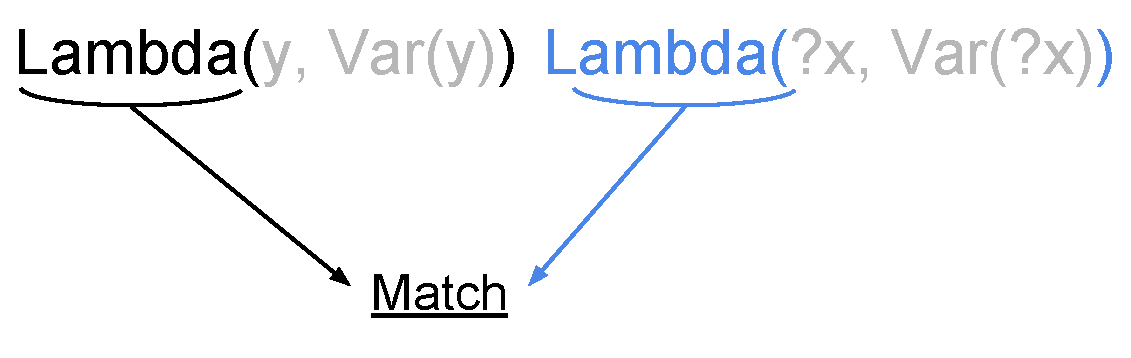
\includegraphics[scale=0.5]{pattern/atom1.pdf}}
  \only<3>
      {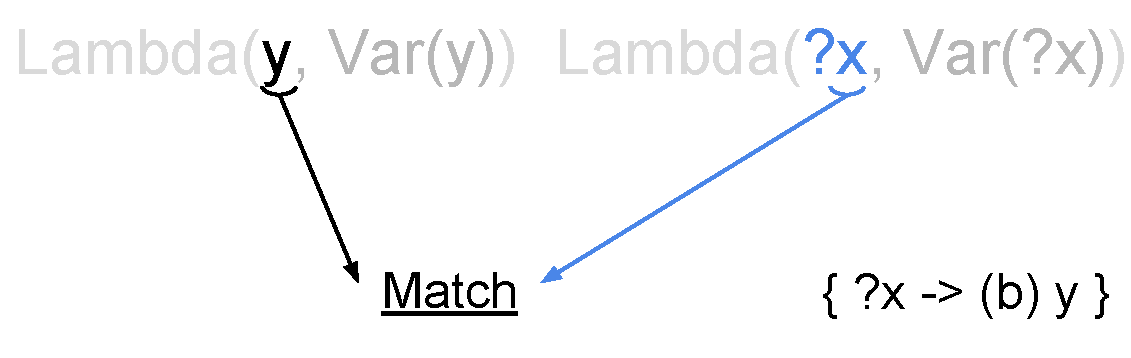
\includegraphics[scale=0.5]{pattern/atom2.pdf}}
  \only<4>
      {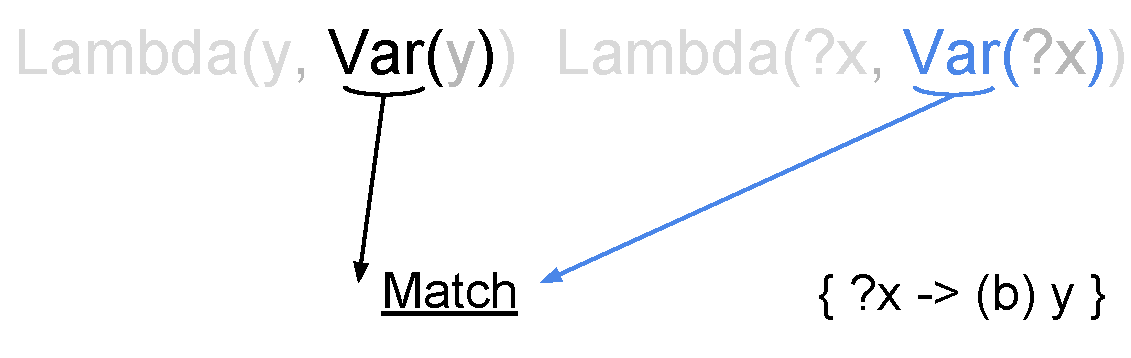
\includegraphics[scale=0.5]{pattern/atom3.pdf}}
  \only<5>
      {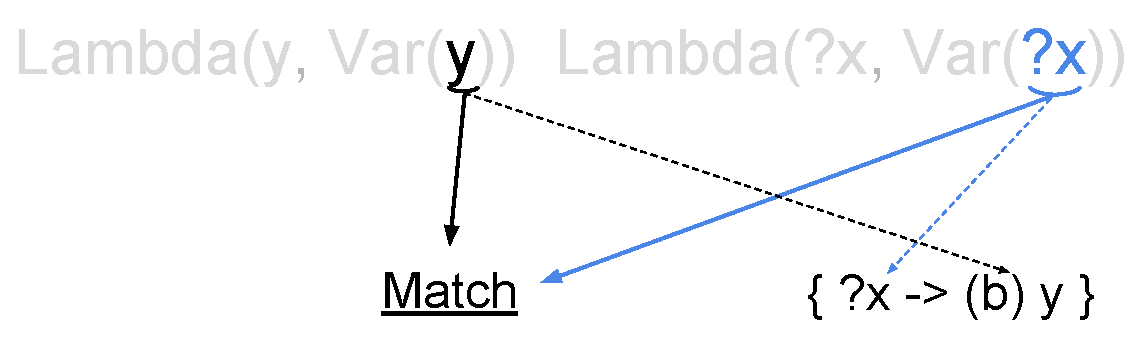
\includegraphics[scale=0.5]{pattern/atom4.pdf}}
  \only<6>
      {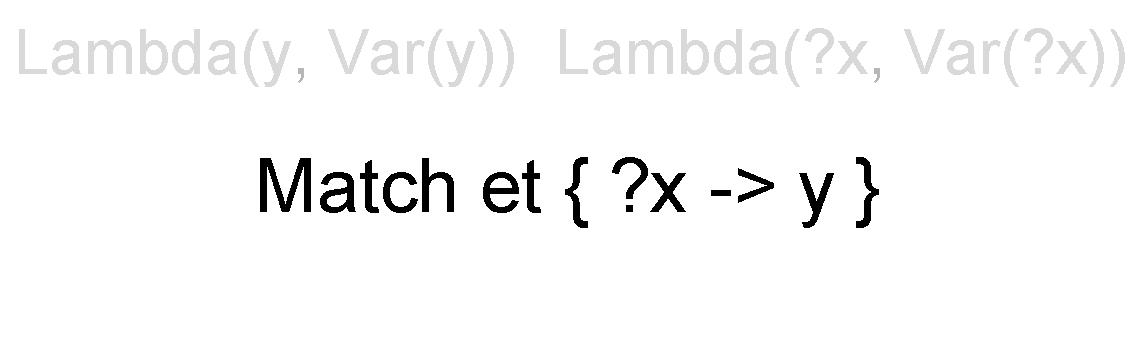
\includegraphics[scale=0.5]{pattern/atom5.pdf}}

\end{center}


\end{frame}

\subsection{Pattern matching non linéaire}

\begin{frame}
\frametitle{Non linéarité avec les termes}

Non linéarité : possiblité d'extraire plusieurs fois le même motif modulo
alpha-conversion.
\begin{itemize}
\item Atomes : possible dans l'algorithme linéaire.
\item Termes : nécessite la capacité de raisonner sur la structure du terme.
\end{itemize}

\bigskip

Exemple :
\begin{itemize}
\item Terme : \texttt{App(Lambda(x, Var(x)), Lambda(y, Var(y)))} matche 
\item Pattern : \texttt{App(?X, ?X)}.
\end{itemize} 

\medskip

Possible puisque le Lambda de droite n'est qu'un renommage du
Lambda de gauche.

\end{frame}

\begin{frame}
\frametitle{Solution : hashconsing}

Une solution élégante permet de régler ce problème : le hashconsing. 

Principe du hashconsing : ne pas allouer deux fois deux structures
identiques. 

\medskip

$\Rightarrow$ Deux termes structurellement identiques seront
le même objet alloué en mémoire.

\bigskip

Le hashconsing des termes fait abstraction des noms de binders et de variables
liées.

\end{frame}

\begin{frame}[fragile]
\frametitle{Hashconsing : exemple d'égalité structurelle}

\begin{columns}
  \column{.5\textwidth}
  Pour le terme 
  \begin{verbatim}
  App(
     Lambda(x, Var(x)), 
     Lambda(y, Var(y))
  )
  \end{verbatim}

  \medskip

  \only<1>{
  
    \column{.5\textwidth}
    Avec hashconsing, l'équivalence structurelle apparait :
    \begin{center}
      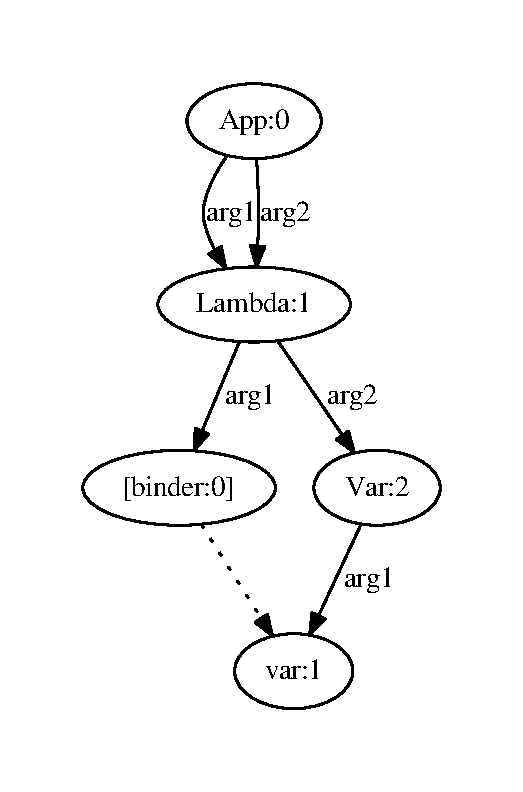
\includegraphics[scale=0.5]{pattern/pres_hash.pdf}
    \end{center}
  }
  
  \only<2>{
  
    \column{.5\textwidth}
    Sans hashconsing :
    \begin{center}
      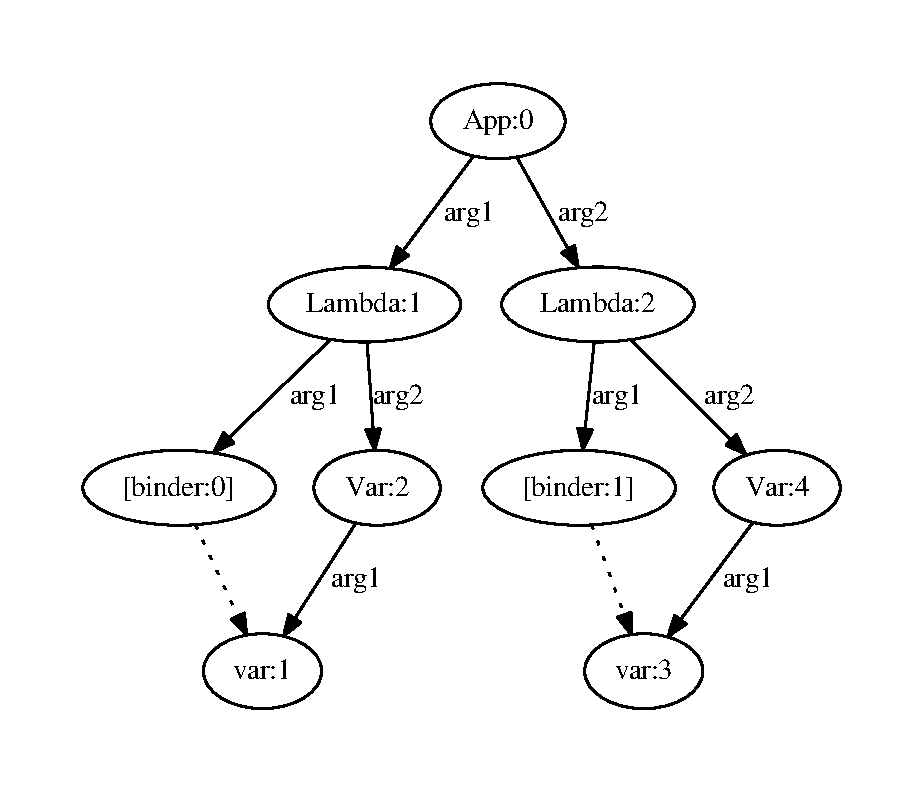
\includegraphics[scale=0.4]{pattern/no_hash.pdf}
    \end{center}
  }
\end{columns}
\end{frame}


%% réécriture / stratégie
%% Roven
\section{Réécriture Nominale}

\begin{frame}{}
\begin{itemize}
\item Pas de contrôles sur l'application des règles ;
\item Besoin d'une solution générique et expressive.
\pause
\item \vspace{0.4cm} Solution : langage de stratégie.
\end{itemize}
\end{frame}

\begin{frame}{Une stratégie}
Une stratégie est une fonction : $ terms * strategies \rightarrow terms $

\begin{itemize}
\item Altération des termes en fonction d'autres stratégies ;
\item Définition d'un nombre minimal de stratégies de bases.
\end{itemize}
\end{frame}

\begin{frame}[fragile]{Stratégies de bases}

{\fontsize{7}{7}

\begin{center}
    \begin{tabular}{ | l | p{6cm}|}
    \hline
    id() & identité \\ \hline
    fail() & toujours en erreur \\ \hline
    test(s) & identité si s reussi \\ \hline
    not(s) & identité si s ne reussi pas \\ \hline
    all(s) & applique s à tout les sous termes \\ \hline
    some(s) & applique s au maximum de sous termes \\ \hline
    one(s) & applique s à au moins un sous terme  \\ \hline
    s1 ; s2 & séquence de s1 puis s2 \\ \hline
    s1 +> s2 & application s1 ou s2 \\ \hline
    s1 + s2 & choix non-dét. : s1 et s2 en parallele \\ \hline 
    proj(n, s) & applique s au nième sous terme \\ \hline
    [r] & applique une règle r \\ \hline
    x & applique la stratégie dans x \\ \hline
    \end{tabular}
\end{center}
}
\end{frame}

\begin{frame}[fragile]{Stratégies par l'utilisateur}
\begin{verbatim}
strategy Topdown(s) :
  s ; all(Topdown(s))

strategy Bottomup(s) :
  all(Bottomup(s)) ; s
\end{verbatim}
\end{frame}

\begin{frame}[fragile]{Stratégies par l'utilistaur}
\begin{verbatim}
strategy Any(s) :
  test(s) +> one(Any(s))

# Any([some_rule])

strategy While(p, s):
  (test(p) ; s ; While(p, s)) +> id()

# si on a : rule [match] :  Foo(?x) -> Foo(?x)

# While(Any([match]), Do_thing)
\end{verbatim}

\end{frame}

\begin{frame}[fragile]{Stratégie de lambda-calcule}

\begin{verbatim}
# the main strategy : 
# - remove all pending substitutions
# - if it's an app ready for beta reduce, apply beta 
#  reduction then loop
# - if it's an app, reduce the right and left then loop
# - if it's a value do nothing
#
strategy ReduceAll :
    SubstAll ;
    (IsAppLambdaValue ; [beta]; ReduceAll) +>
    (IsApp ; Left(ReduceAll) ; 
      Right(ReduceAll) ; ReduceAll) +>
    (IsValue ; id())
\end{verbatim}

\end{frame}

\begin{frame}{}
\begin{itemize}
\item Système satisfaisant ;
\item Contrôle fin de l'application des règles ;
\item Bonne expressivité.
\end{itemize}
\end{frame}


%% utilisation du bouzin
%% Vincent
\section{Mode Interactif}
\begin{frame}{Toplevel}

\begin{block}{Mode interactif}
Permet à l'utilisateur de manipuler directement le système en rajoutant règles,
stratégies ou encore la réduction directe de terme.
\end{block}

\begin{block}{Directives}
\begin{itemize}
\item Effectuer des tests sur une expression selon plusieurs modalités
\item Afficher le type d'un terme
\item Exporter la représentation d'un terme \emph{hash-consé} vers un graphe
\end{itemize}
\end{block}

\end{frame}

\begin{frame}[fragile]{Tests}

\begin{block}{Tester les termes}
\begin{verbatim} 
:test <terme> <predicat> <resultat> 
\end{verbatim}
\end{block}

Tester l'addition dans le système de réécriture des axiomes de Peano :
\begin{verbatim}
:test rewrite Add(Successor(Zero), Successor(Zero)) 
      with BottomupAll --equal Successor(Successor(Zero))
\end{verbatim}

\end{frame}

\begin{frame}[fragile]{Test d'une erreur}

Nous pouvons également tester l'échec d'un test par une erreur pré-définie :
\medskip

\begin{verbatim}
:test Successor(Zero, Zero) 
      --failwith TermSystemError.WrongTermArity
\end{verbatim}

\end{frame}

\begin{frame}[fragile]{Test alpha-conversion}
  On peut aussi tester la correspondance d'un terme à un type ou à un
  pattern.

\begin{block}{Alpha-conversion dans le lambda-calcul}
\begin{verbatim}
:match App(Lambda(x, Var(x)), Lambda(y, Var(y))) 
       --with App(?T, ?T) 
\end{verbatim}
\end{block}

\end{frame}

\begin{frame}{Directives utilitaires}

  \begin{itemize}
  \item \textt{:type <t>} -- Permet d'afficher le type du terme t
  \bigskip

  \item \textt{:dot <t> <fichier>} -- Crée un graphe ``dot'' de la version \emph{hash-consé} du term t
  \end{itemize}

\end{frame}


%% démo
%% Pierre Roven
\section{Démonstration}
\input{demo.tex}


%% Bilan

%% partie chiante pour Pierre
%% Pierre Inigo
\section{Bilan}
%% Ce qu'on a appris en pratique et en théorie
  %% méthode agile
  %% OCaml
  %% outils gestion de projet
  %% système de réécriture

%% Ce qu'on a fait

%% Ce qui n'a pas bien fonctionné / Ce qu'il aurait fallu changer


\end{document}
